
%(BEGIN_QUESTION)
% Copyright 2015, Tony R. Kuphaldt, released under the Creative Commons Attribution License (v 1.0)
% This means you may do almost anything with this work of mine, so long as you give me proper credit

\noindent

\vskip 5pt

\vskip 5pt
\begin{center}
\vskip 5pt 
\textbf{Industrirobot -- Nivå 1 }
\vskip 5pt 
\textbf{Arbidsoppdrag på egen PC}
\vskip 5pt 
\textbf{Grunnleggende om robot}
\end{center}

\vskip 5pt 
I dette oppdraget trenger du to ulike robotstasjoner til robotstudio. Disse finner du her:

\vskip 5pt 
\href{https://rfka-my.sharepoint.com/:u:/r/personal/fred-olav_mosdal_skole_rogfk_no/Documents/ForAutofaget.no/Robotstasjon1.rspag?csf=1&web=1&e=Zm7EG9}{Robotstasjon1}

\vskip 5pt 
\href{https://rfka-my.sharepoint.com/:u:/r/personal/fred-olav_mosdal_skole_rogfk_no/Documents/ForAutofaget.no/Robotstasjon2.rspag?csf=1&web=1&e=kk7j4H}{Robotstasjon2}

\vskip 5pt 
\textbf{Arbeidsoppdrag - Jogging og TCP}

\textbf{Jogging}

\vspace{1cm}

For å komme til jogge vindu trykker du følgende:

\vspace{1cm}

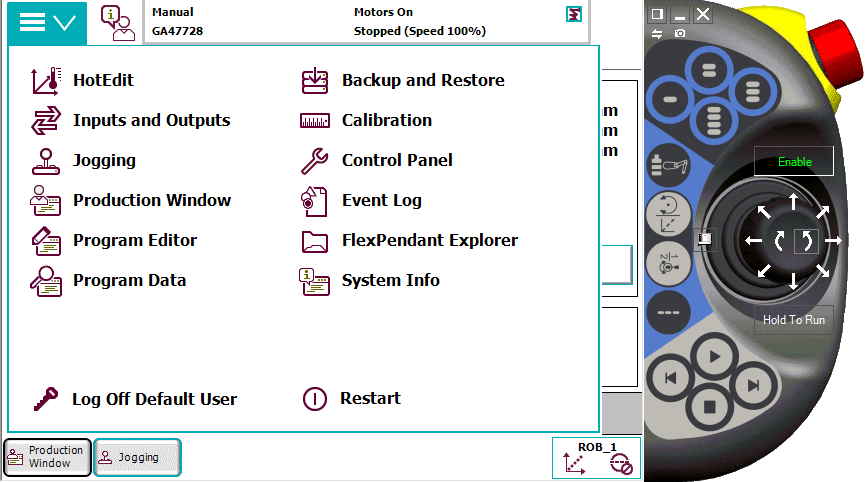
\includegraphics[width=0.5\textwidth]{i04861x01}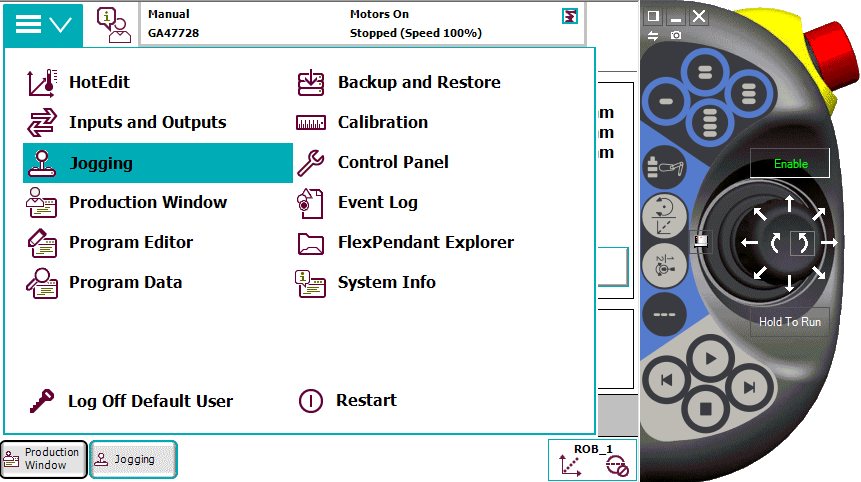
\includegraphics[width=0.5\textwidth]{i04861x02}

\vspace{1cm}

Prøv ut de forskjelleige Motion Mode: Axis 1 - 3, Axis 4-6, Linear og Reorient. Finn ut hva som er forskjellen og forbred deg på å forklare for andre denne forskjellen. 

\vspace{1cm}

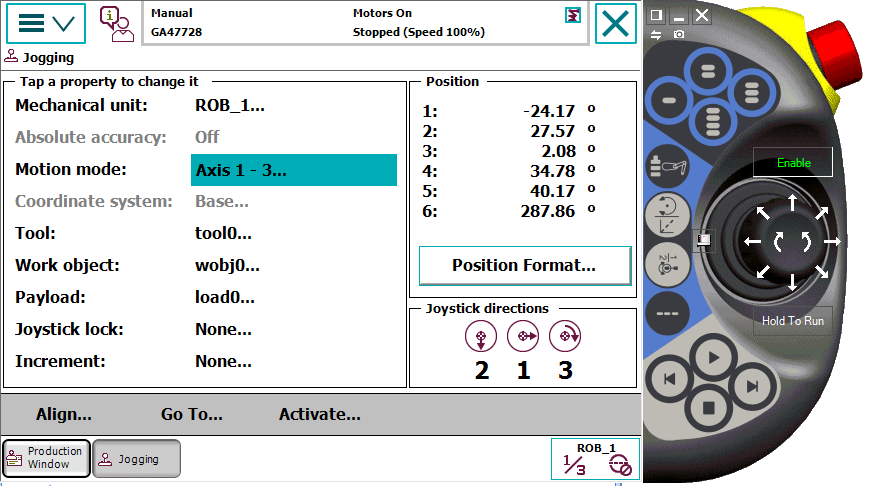
\includegraphics[width=1\textwidth]{i04861x03}

\vspace{1cm}

Jogg robot i forskjellige koordinatsystem, Base/ tool/Workobject. Finn ut hva som er forskjellen og forbred deg på å forklare for andre denne forskjellen. 

\vspace{1cm}

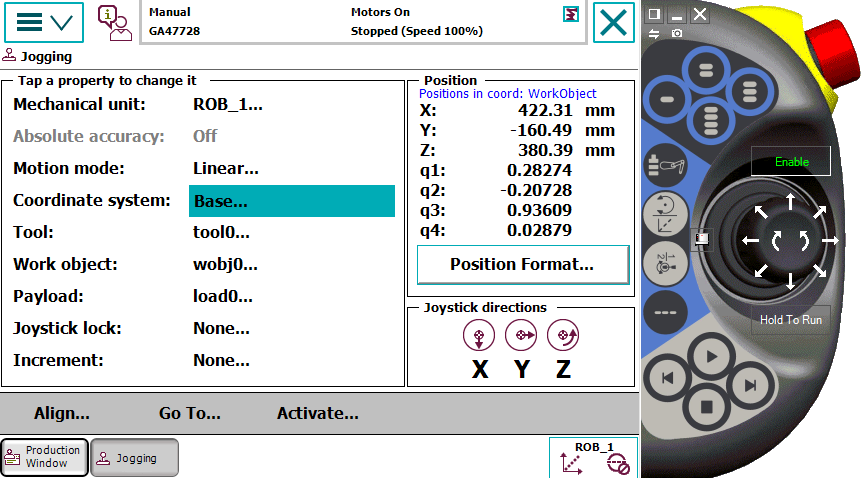
\includegraphics[width=1\textwidth]{i04861x04}

\vspace{1cm}

Align robot vil rette verktøyet ut bruker mot den nærmeste aksen x, y eller Z. Prøv ut denne funksjonen. 

\vspace{1cm}

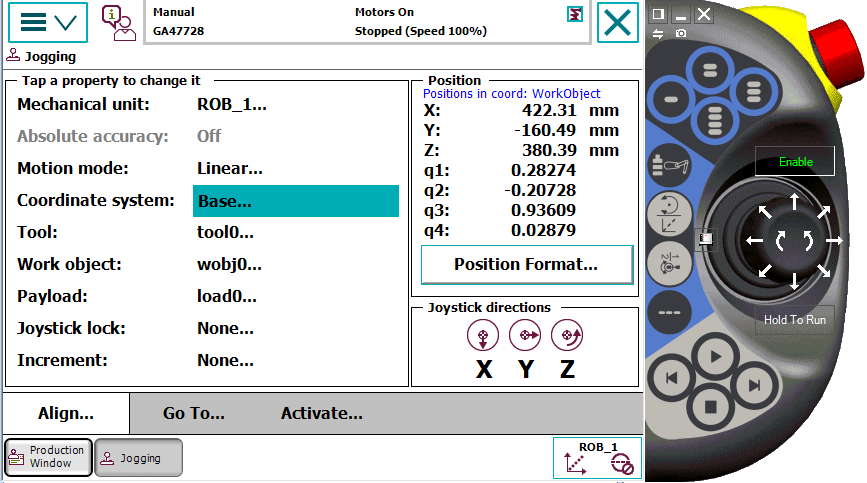
\includegraphics[width=1\textwidth]{i04861x05}

\vspace{1cm}

Hvilken annen informasjon får du fra jogge vinduet?

\vspace{1cm}


\textbf{TCP (Tool Center Point)}

\vspace{1cm}

Mål: Lære å opprette TCP manuelt og ved hjelp av robot.
\vskip 5pt 
Å sette tool center point er en måte å gjøre roboten klar  ovor senter på verkøyet du bruker er. For å plassere verktøyer er vi helt avhengig av at dette er definert. 

\vspace{1cm}

Velg program data og velg tooldata

\vspace{1cm}

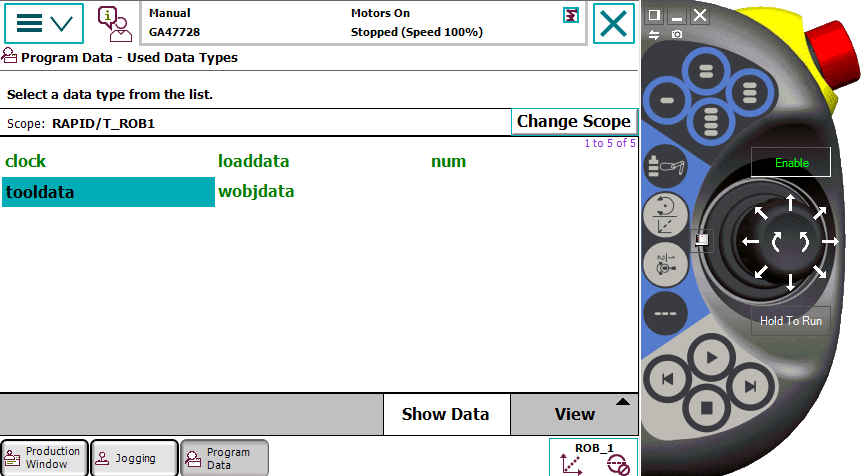
\includegraphics[width=1\textwidth]{i04861x06}

\vspace{1cm}

Trykk på new.

\vspace{1cm}

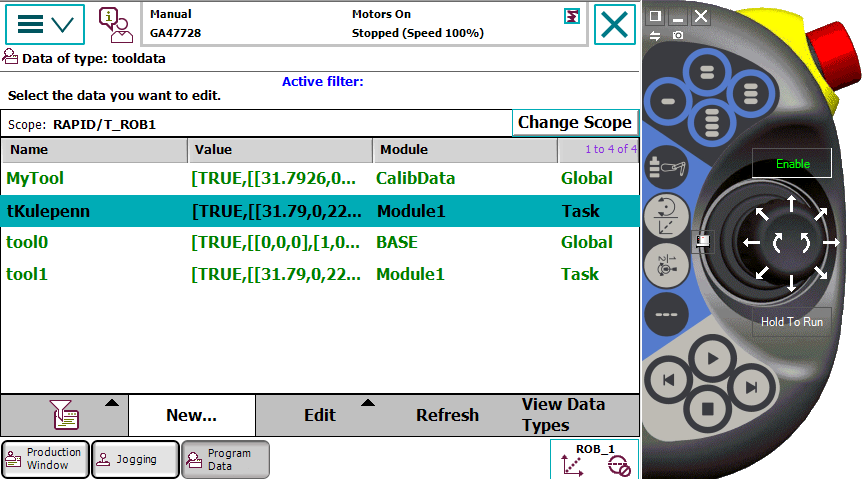
\includegraphics[width=1\textwidth]{i04861x07}

\vspace{1cm}

Vi kaller TCP \textquoteleft en «tKulepenn2». Sørg for at du velger
samme alternativ som på bildet.

\vspace{1cm}

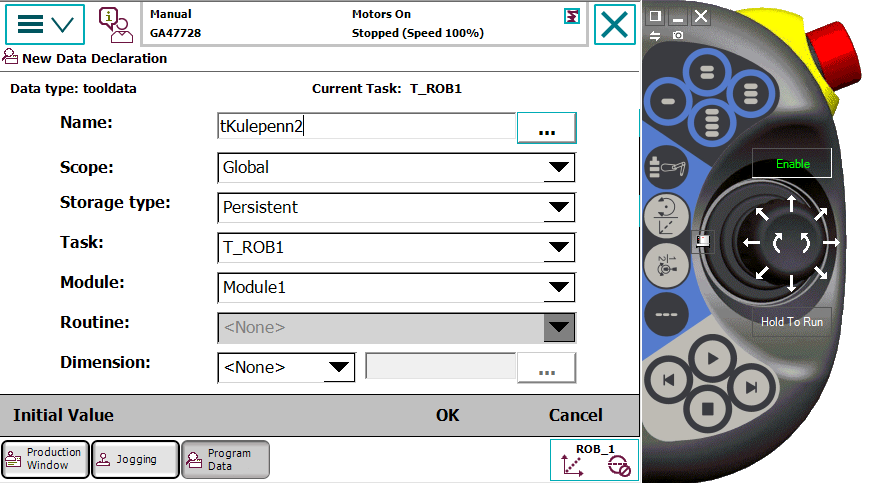
\includegraphics[width=1\textwidth]{i04861x08}

\vspace{1cm}

Vi skal nå legge inn avstanden fra flens på robot til tuppen av kulepennen. 

Trykk OK.

\vspace{1cm}

Velg Inital Value og legg inn følgende verdier:
\begin{itemize}
\item Toolframe Z = 70 (mm) og X = 130 (mm). 
\item Mass = 1 kg. 
\item COG Z= 100 mm.
\end{itemize}
NB! Dersom enn glemmer å definere vekt og COG, vil du ikke kunne bruke
det aktuelle «tool»

\vspace{1cm}

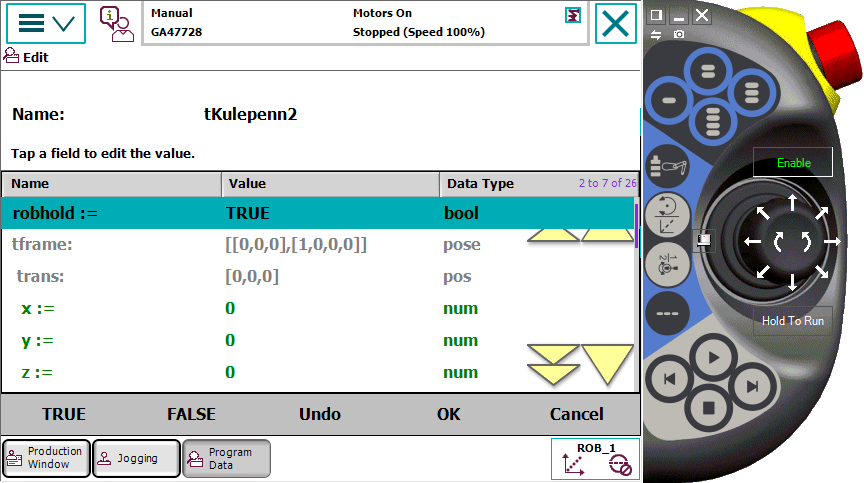
\includegraphics[width=1\textwidth]{i04861x09}

Trykk OK

Jog roboten I reorient og se hvordan det virker

\vspace{1cm}


\textbf{Definer tcp ved hjelp av robot (4punkt).}

\vspace{1cm}

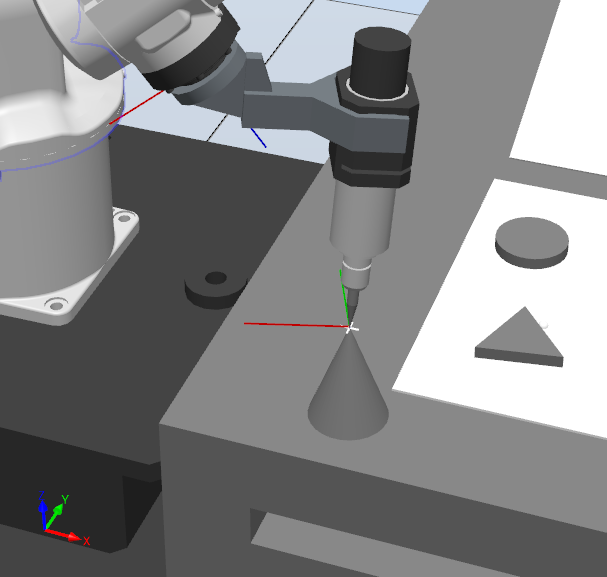
\includegraphics[width=1\textwidth]{i04861x10}

\vspace{1cm}

Marker tKulepenn2, trykk edit og velg define.

\vspace{1cm}

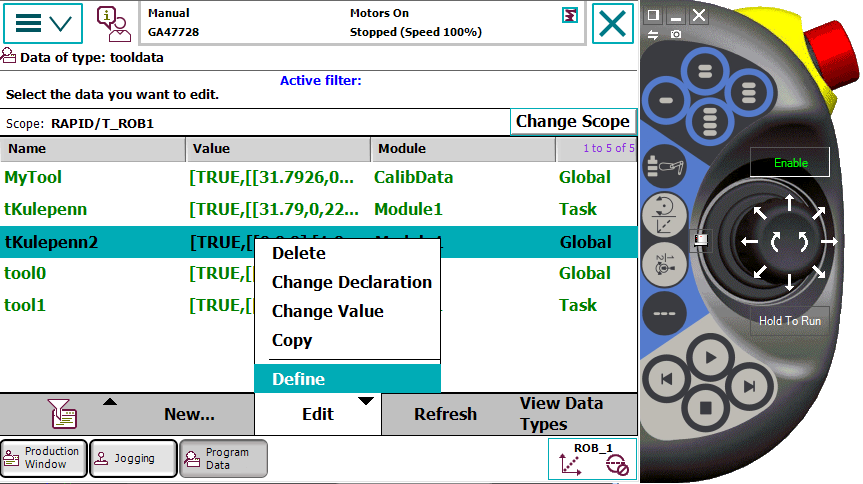
\includegraphics[width=1\textwidth]{i04861x11}

\vspace{1cm}

Jog robot spiss mot spiss på 4 forskjellige måter (se første bilde
i oppgave) Størst vinkel mellom punktene vil gi den mest nøyaktige
TCP.

Husk å trykk «modify position» for hver gang du står spiss mot spiss.

\vspace{1cm}

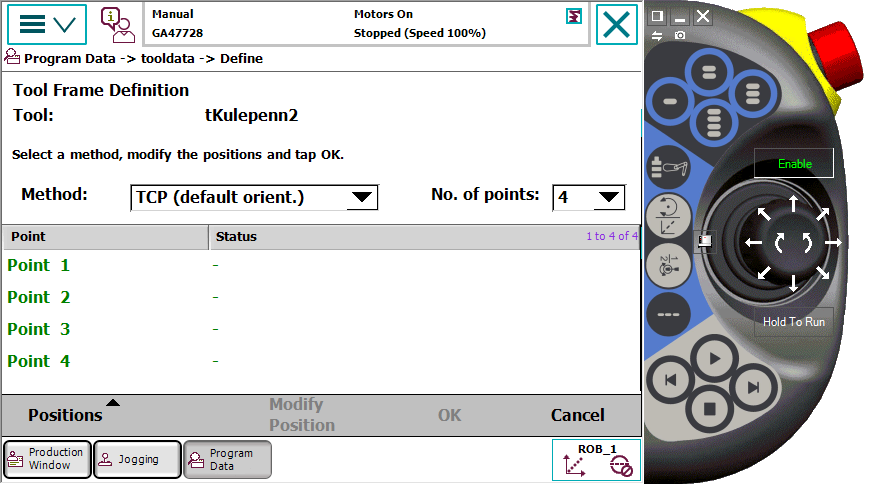
\includegraphics[width=1\textwidth]{i04861x12}

\vspace{1cm}

Når du har satt alle 4 posisjonene, trykk OK.

\vspace{1cm}

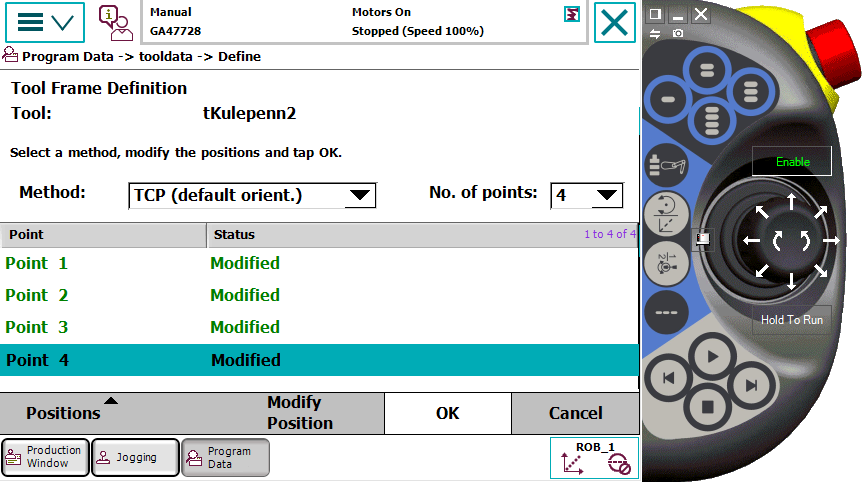
\includegraphics[width=1\textwidth]{i04861x13}

Robot vil nå kalkulere krysningspunkt for alle posisjonene, og lage
en TCP ut av resultatet.

\vspace{1cm}

TIPS! Etter du har trykket OK, vil du få opp en side som gir deg alle
de utregna verdiene. Mean error bør være under 0,5, da har du en nøyaktig
TCP.

\paragraph{Sjekk: Lærer sjekker om eleven kan utføre:}
\begin{itemize}
\item Jogging
\item Bytte av workobjekt
\item Reorientering av tool
\item Align av tool
\item Vise at reorient virker på tool om elev har laget selv.
\end{itemize}


\textbf{Arbeidsoppdrag 2 - Workobject og bevegelser}

\textbf{Workobject}

Mål: Lære å opprette ett work object, og definere origo (nullpunkt)

\includegraphics[width=1\textwidth]{../nogpl/i04861x14}

Velg program data i hovedmeny, trykk deretter på wobjdata.

Velg new

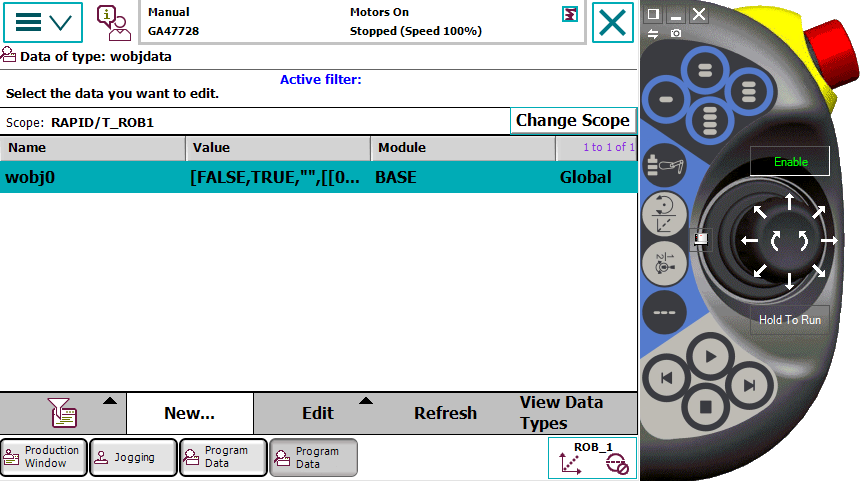
\includegraphics[width=1\textwidth]{i04861x15}

3. Vi velger å kalle work objectet «wobjArk».

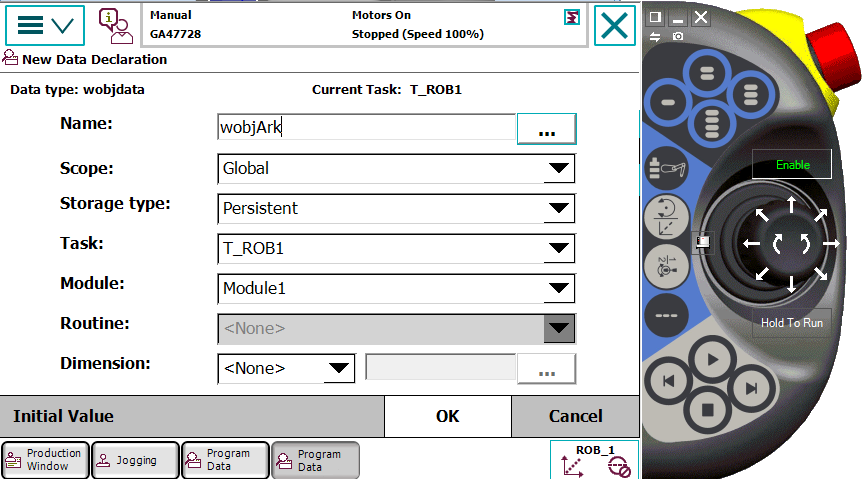
\includegraphics[width=1\textwidth]{i04861x16}

Trykk OK 

Vi skal nå definere null punktet. Marker wobjArk, trykk på Edit, og
velg Define.

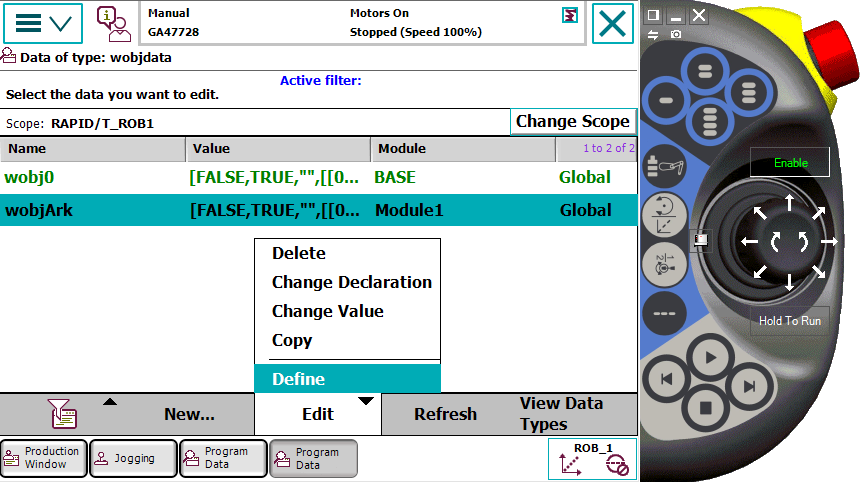
\includegraphics[width=1\textwidth]{i04861x17}

Velg 3 points både på «User method» og «Object method»

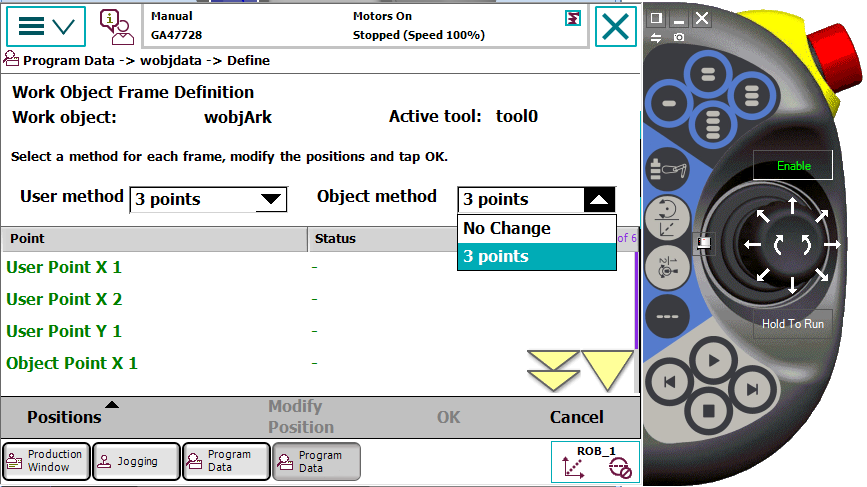
\includegraphics[width=1\textwidth]{i04861x18}

Vi skal nå definere origo for work objectet, jog robot til X1, marker User point X1 og trykk Modify position. I samme position trykk modify position for object point X1.

Repeter for X2 og Y1.

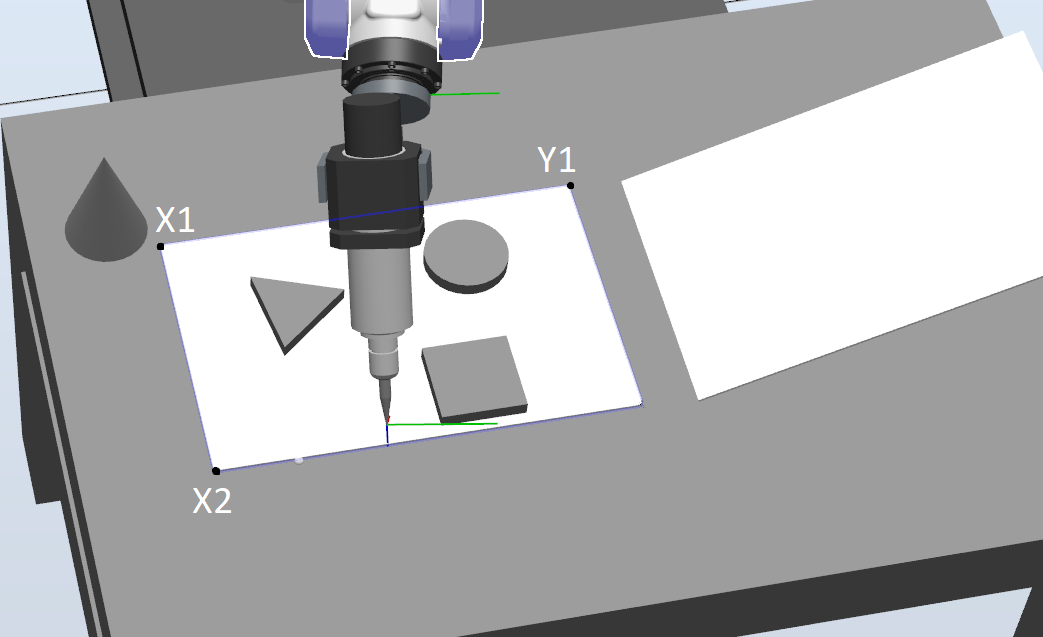
\includegraphics[width=1\textwidth]{i04861x19}

Trykk OK 

Jogg robot etter workobject.

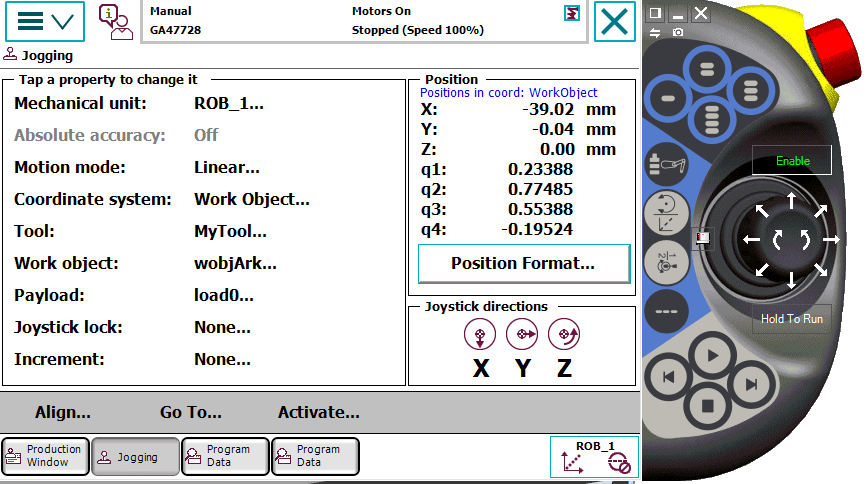
\includegraphics[width=1\textwidth]{i04861x20}

«Align» robot etter workobject

Lag ett nytt workobject på en skrå flate (For eksempel en perm). 

Jogg robot etter workobject OBSERVER. 

«Align» robot etter workobject.

\textbf{Bevegelser}

Mål: Lære bruk og forskjell på MoveL og MoveJ.

Roboten skal nå kjøre lineært fra en posisjon (p10) til en annen (p20),
og deretter tilbake med en MoveJ bevegelse.

Bevegelsen vil se slik ut:

\includegraphics{../nogpl/i04861x21}

Jog robot til startposisjon, og sørg for at både tKulepenn og wobjArk
er aktivt. 

Velg Program editor i hovedmeny. Marker <smt> og trykk Add instruction

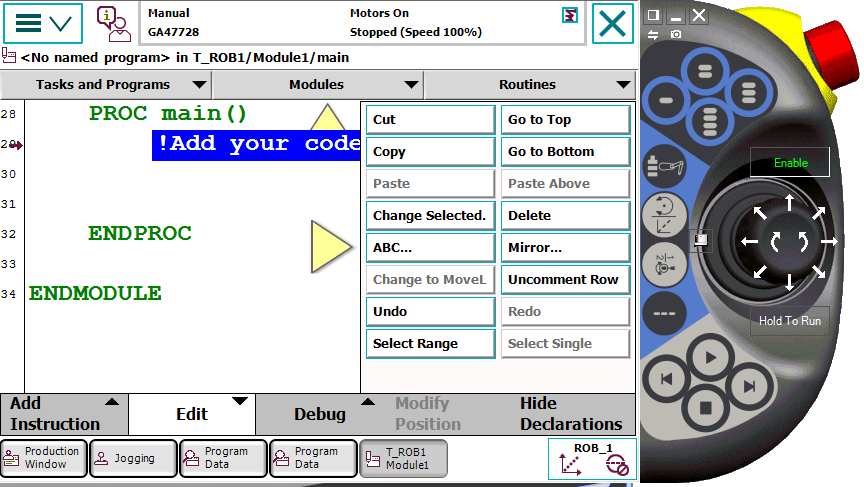
\includegraphics[width=1\textwidth]{i04861x22}

Velg instruksjonen MoveL

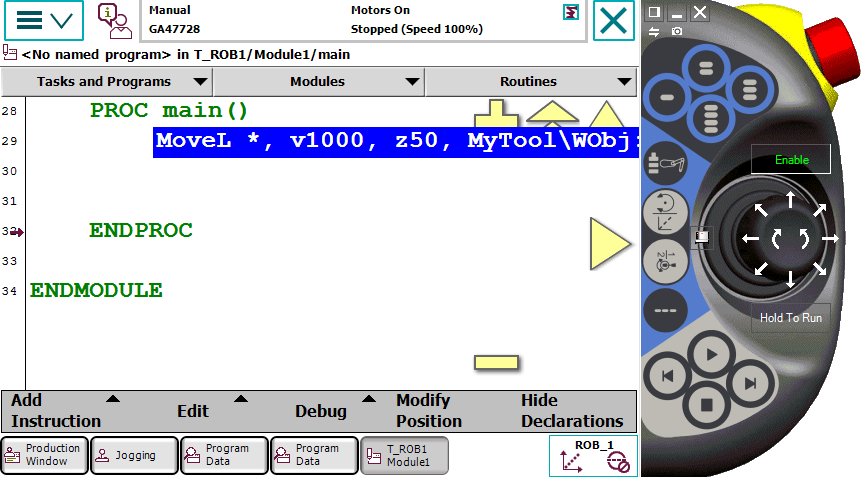
\includegraphics[width=1\textwidth]{i04861x23}

Dobbel klikk på stjernen for å endre navn. Velg new, roboten vil automatisk
foreslå p10.

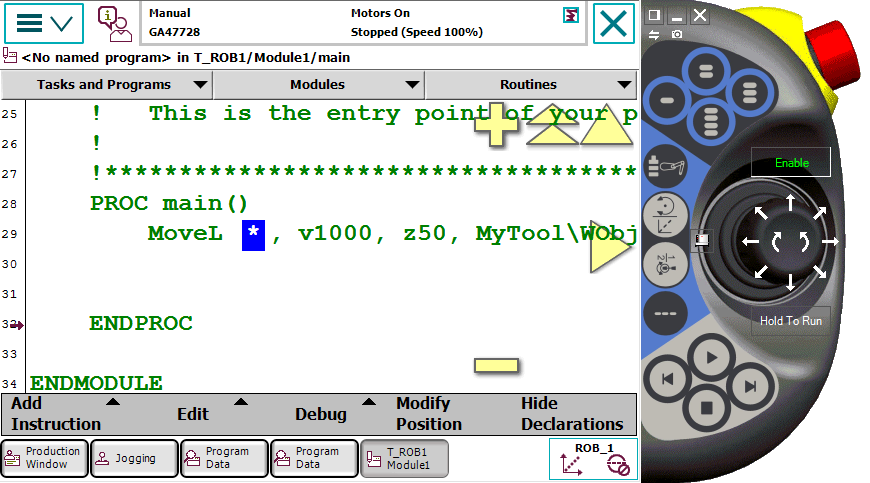
\includegraphics[width=1\textwidth]{i04861x24}

Trykk OK.

Jogg til et punkt 20cm fra p10.

Lag et punkt p20 på arket.

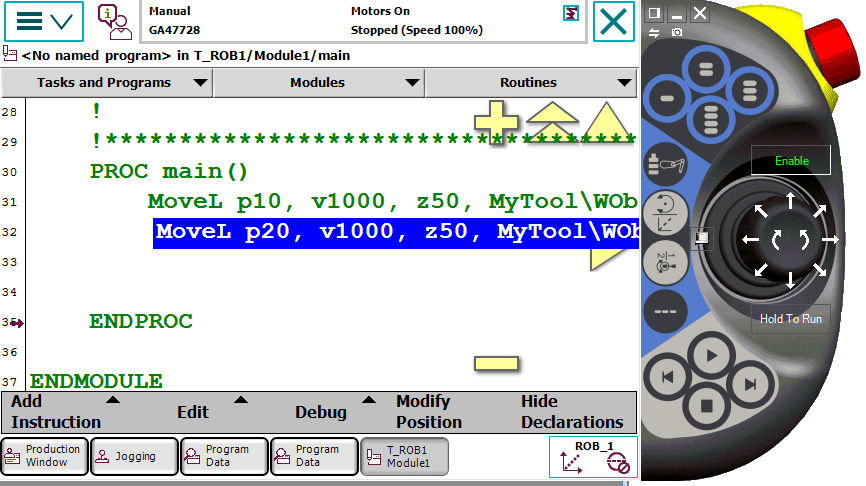
\includegraphics[width=1\textwidth]{i04861x25}

Kjør tilbake til punkt p10, men denne gang med instruksjonen MoveJ

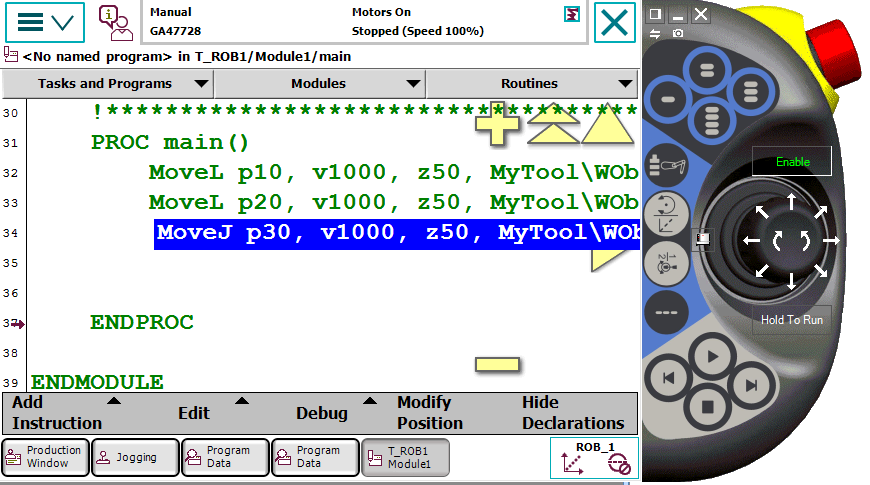
\includegraphics[width=1\textwidth]{i04861x26}

For å teste programmet trykk «debug», deretter «PP to Main». Nå kan
robot startes ved å holde inne «live handle» knapp og trykke play
knapp.

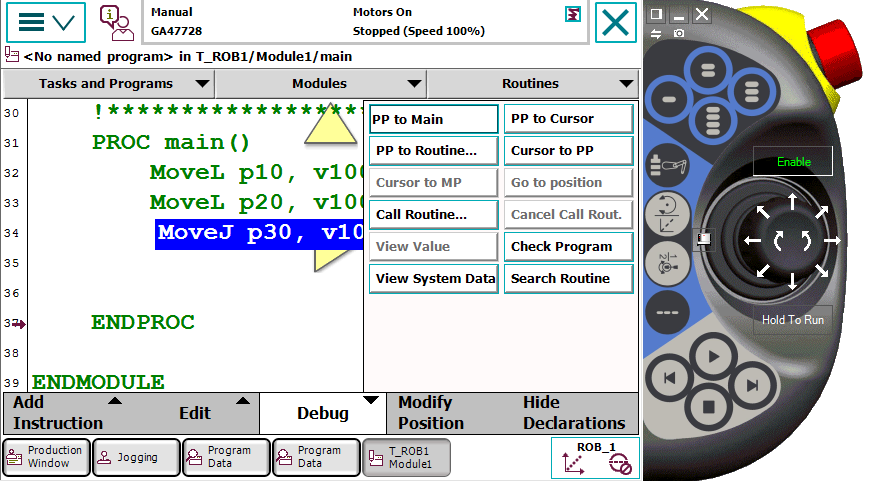
\includegraphics[width=1\textwidth]{i04861x27}

PP to Main betyr program peker til start

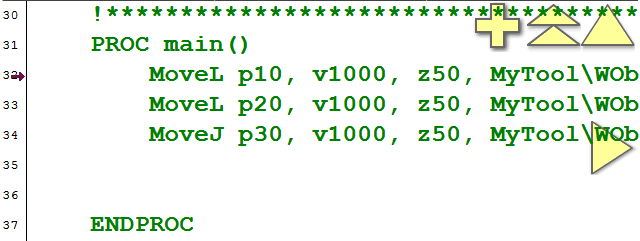
\includegraphics[width=1\textwidth]{i04861x28}

Pilen visualiserer hvor i programmet enn er.

Observer hva som skjer.

Hva består en MoveL og MoveJ instruksjon av? 

Robtarget: består av X,Y,Z koordinat samt kvaternioner q1-q4 som oppgir
orienteringen. Ett robtarget kan enten være ett «stjernepunkt» eller
gis individuelt navn. 

Speeddata: hastigheten roboten skal kjøre til punktet med. For eksempel
V1000 som vil si 1000mm/s. 

Zonedata: Avgjer når robot kan begynne på neste instruksjon og bane.
Dersom du har en sone på z100, kan robot begynne å kjøre mot neste
punkt 100mm før den har nådd punktet. 

\includegraphics[width=1\textwidth]{../nogpl/i04861x29}

Tooldata: koordinat system ut fra flens på robot.

\includegraphics{../nogpl/i04861x30}

Work object: Egen definert koordinatsystem.

\textbf{Figurer}

Mål: Lære å lage rutiner, bruke instruksjonen MoveC og endre hastighet
/soner i instruksjoner. 

Først og fremst skal vi opprette 3 nye rutiner. Firkant, trekant og
sirkel. 

Trykk på Routines. 

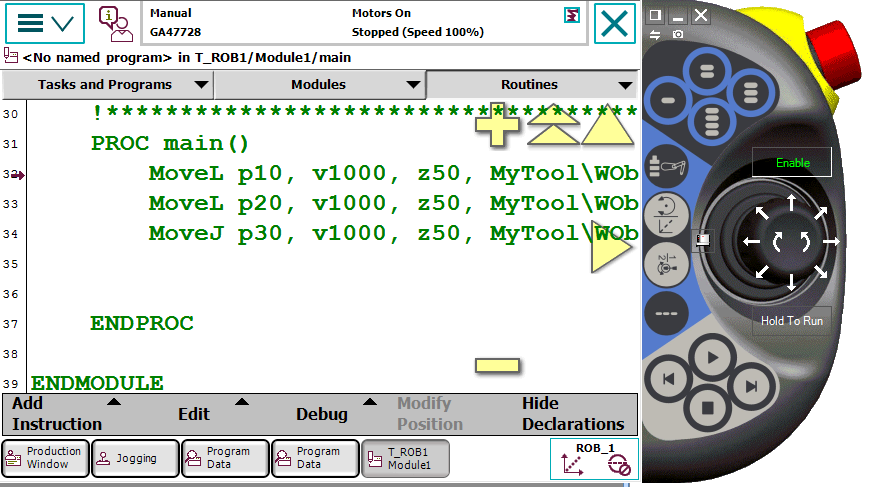
\includegraphics[width=1\textwidth]{i04861x31}

Velg File og new routine 

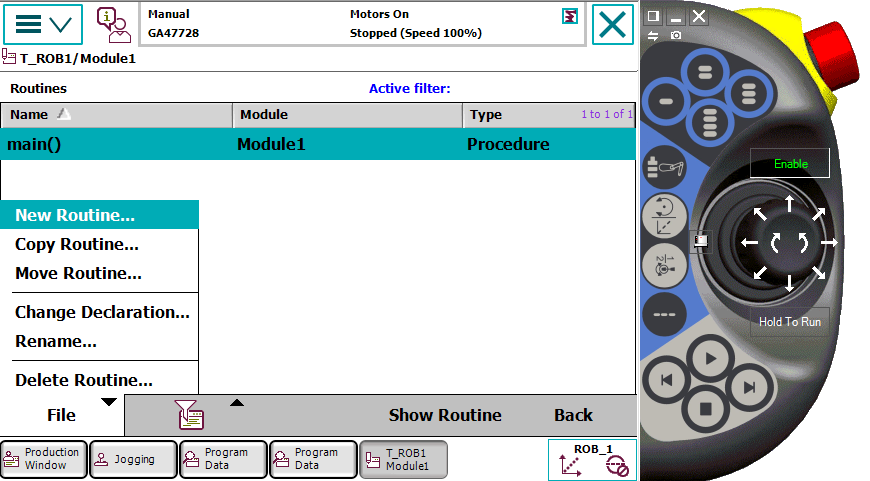
\includegraphics[width=1\textwidth]{i04861x32}

Opprett 3 rutiner, firkant, trekant og sirkel. 

Lag program for å tegne firkant, trekant og sirkel. For å lage sirkel
bruker vi instruksjonen MoveC. Se eksempel. 

\includegraphics{../nogpl/i04861x33}

For å kjøre en enkel rutine velg debug, og PP to Routine. 

Prøv å endre hastighet på de forskjellige instruksjonene. (under 250mm/s) 

Prøv å endre zonedata. 

Observer hva som skjer. 

for å kjøre alle rutiner automatisk må de legges inn i Main rutinen.
Vi sletter først alt gammelt i main. 

For å kalle opp rutiner brukes instruksjonen ProcCall. Main rutinen
skal se slik ut: 

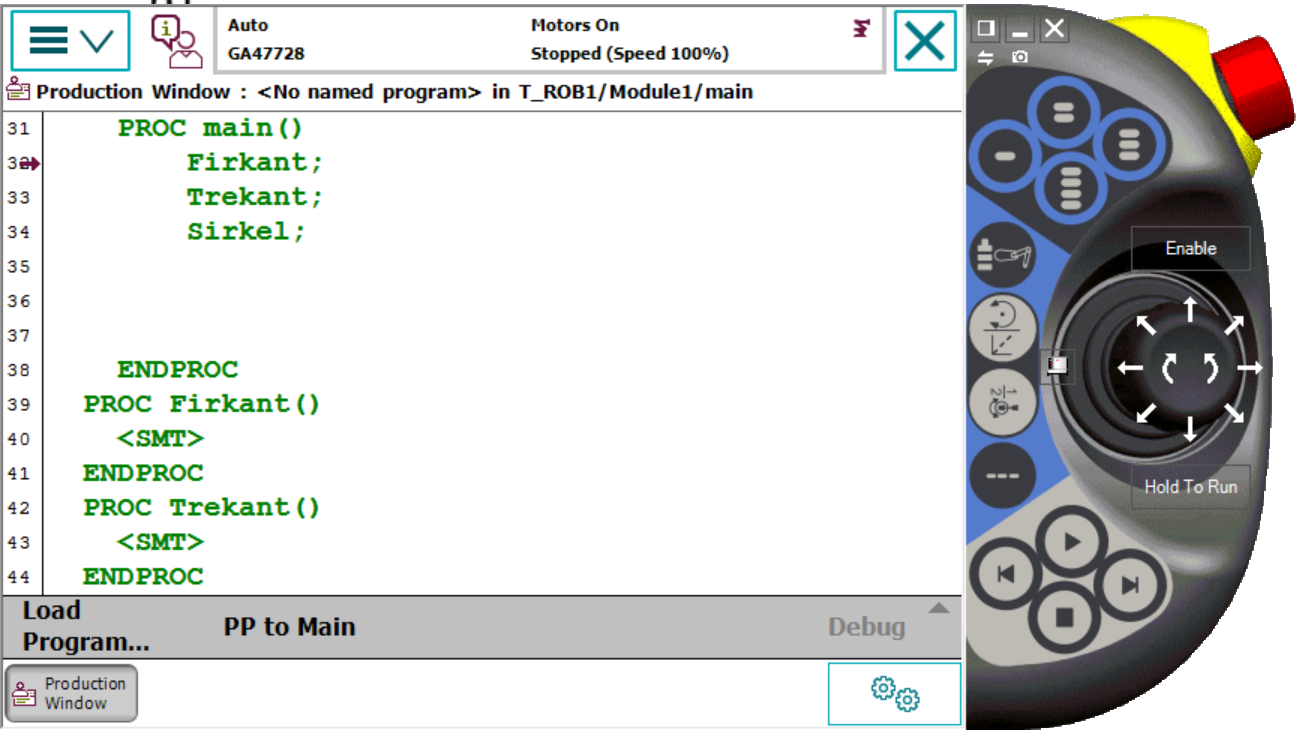
\includegraphics[width=1\textwidth]{i04861x34}

\textbf{Flytte WorkObject}

Mål: Lære forskjell på «userframe» og «objectframe» . 

Bruk program fra oppg 5. 

Gå til program data 

Velg wobjdata 

Dobbelklikk på wobjArk 

Forflytt userframe 50 mm i X retning. 

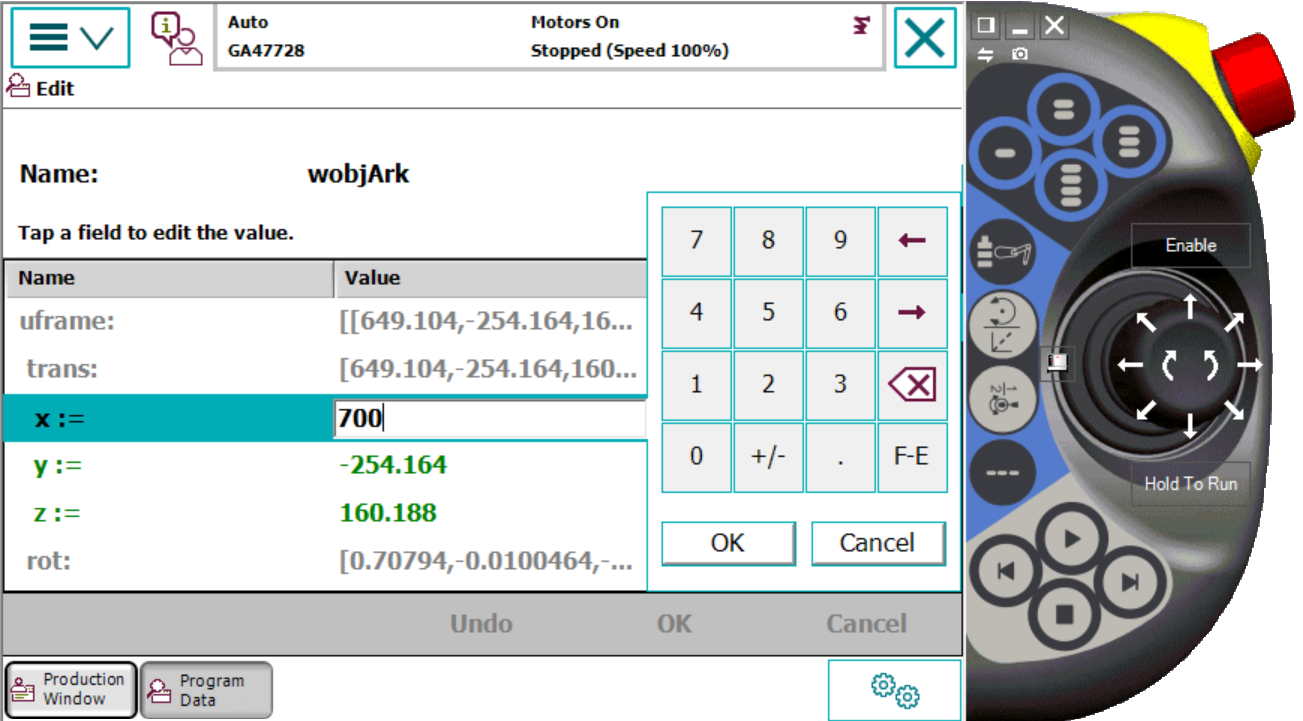
\includegraphics[width=1\textwidth]{i04861x35}

Kjør program og observer hva som skjer. 

Legg inn gamle verdier i userframe. Forflytt så objectframe 50mm i
X retning. 

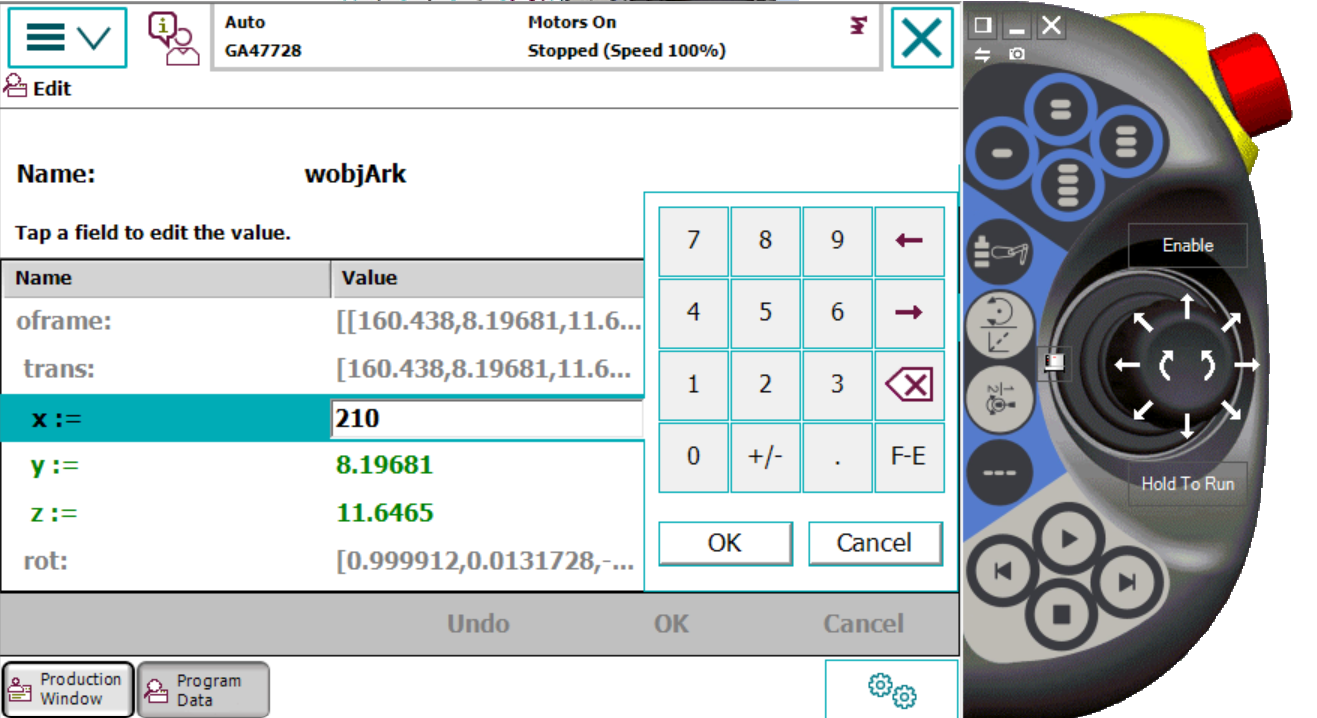
\includegraphics[width=1\textwidth]{i04861x36}

Kjør program og observer hva som skjer. 

\textbf{Arbeidsoppdrag 3 - Programmering I}

\textbf{IF instruksjonen}

Mål: Forstå bruk av IF instruksjonen.
\begin{enumerate}

\item Lag ett program hvor du bruker bryterne til å bestemme hvilken figur
som skal tegnes. Sett opp main rutinen ved hjelp av instruksjonen
IF.

diBr står for digital input Bryter. Ett digitalt inngangssignal er
i bunn og grunn ett 24 V signal som er koblet til IO kortet til roboten.
Dette signalet vil enten være 1 eller 0 ut ifra om bryteren er på
eller av.

Eks.
\begin{lstlisting}[basicstyle={\sffamily}]
PROC main()
	IF diBr1=1 THEN
		Trekant;
	ELSEIF diBr2=1 THEN
		Sirkel;
	ELSEIF diBr3=1 THEN
		Firkant;
	ENDIF
ENDPROC
\end{lstlisting}

\end{enumerate}

\textbf{WHILE instruksjonen}

Mål: Forstå bruk av WHILE instruksjon
\begin{enumerate}
\item Bruk WHILE til å velge mellom trekant, firkant og sirkel.

Eks.
\begin{lstlisting}[basicstyle={\sffamily}]
PROC main()
	WHILE diBr1=1 do
		Trekant;
	ENDWHILE
	WHILE diBr2=1 do
		Firkant;
	ENDWHILE
	WHILE diBr3=1 do
		Sirkel;
	ENDWHILE  
ENDPROC
\end{lstlisting}

\end{enumerate}

\textbf{FOR instruksjonen}

Mål: Forstå bruk av FOR instruksjon
\begin{enumerate}
\item Bruk FOR til å velge antall sykluser

Eks.

\begin{lstlisting}[basicstyle={\sffamily}]
PROC main()
	FOR i FROM 1 TO 5 DO
		Trekant;
	ENDFOR
	FOR i FROM 1 TO 3 DO
		Firkant;
	ENDFOR
	FOR i FROM 1 TO 2 DO
		Sirkel;
	ENDFOR   
ENDPROC
\end{lstlisting}

i står for Identifier (iterator), og er en ren teller.
\end{enumerate}

\textbf{TEST instruksjonen}

Mål: Forstå bruk av TEST instruksjon
\begin{enumerate}
\item Bruk TEST til å velge syklys.

For å kunne bruke TEST instruksjonen må vi opprette ett register/num.
Det er en type program data som husker tallet den har blitt gitt.
\item Gå til program data og velg num.
\item Trykk new og gi registeret navnet nFigur. 

For å endre verdi på nFigur, gå til program data num og velg nFigur.
Du vil da få mulighet til å endre tallet. 

Dersom tallet er verken 1,2, eller 3 vil program peker hoppe til default.

Eks.

\begin{lstlisting}[basicstyle={\sffamily}]
PROC main()
TEST nFigur   
	CASE 1:
		Trekant
	CASE 2:
		Firkant;
	CASE 3:
		Sirkel;
	DEFAULT:
		Stop;
	ENDTEST    
ENDPROC
\end{lstlisting}

\end{enumerate}


\textbf{Operatørkommunikasjon}

Mål: Lære å bruke TPReadFK og TPReadNum.

Du skal nå bruke det du har lært til å lage ett program som spør hvilken
figur som skal tegnes, og hvor mange ganger den skal tegnes.
\begin{enumerate}
\item 1. Lag Init rutine der du nullstiller register og åpner griper. -

Instruksjonen := kan brukes til å nullstille registeret, eller å gi
det den verdien du ønsker.

\begin{lstlisting}[basicstyle={\sffamily}]
PROC init()
	reg1 := 0;
	Reset CloseClaw; 		
	Set OpenClaw;
ENDPROC
\end{lstlisting}

\item Lag Meny rutine hvor instruksjonene TPReadFK skal brukes for å bestemme
hvilken figur som skal tegnes, og TPReadNum for å bestemme antall
ganger figuren skal tegnes.

Beskrivelse av TPReadFK:

TPReadFK (FlexPendant Read Function Key) er brukt til å skrive tekst
på funksjons knappene, og til å finne ut hvilken knapp som trykkes
på.

Eksempel 1

\begin{lstlisting}[basicstyle={\sffamily}]
TPReadFK reg1, "More?", stEmpty, stEmpty, stEmpty, "Yes", "No"; 
\end{lstlisting}

Teksten More? Blir skrevet på flexpendant skjermen, samt knappene
4 og 5 er aktivert med tekstene \textquotedblleft Yes\textquotedblright{}
og \textquotedblleft No\textquotedblright{} (se bildet nedenfor).
Programmet vil ikke gå videre før eventuelt knapp 4 eller 5 trykkes
på. Med andre ord, reg1 vil få verdien 4 eller 5 avhengig av hvilken
knapp som trykkes på. 

Bildet illustrerer hvordan instruksjonen vil se ut.

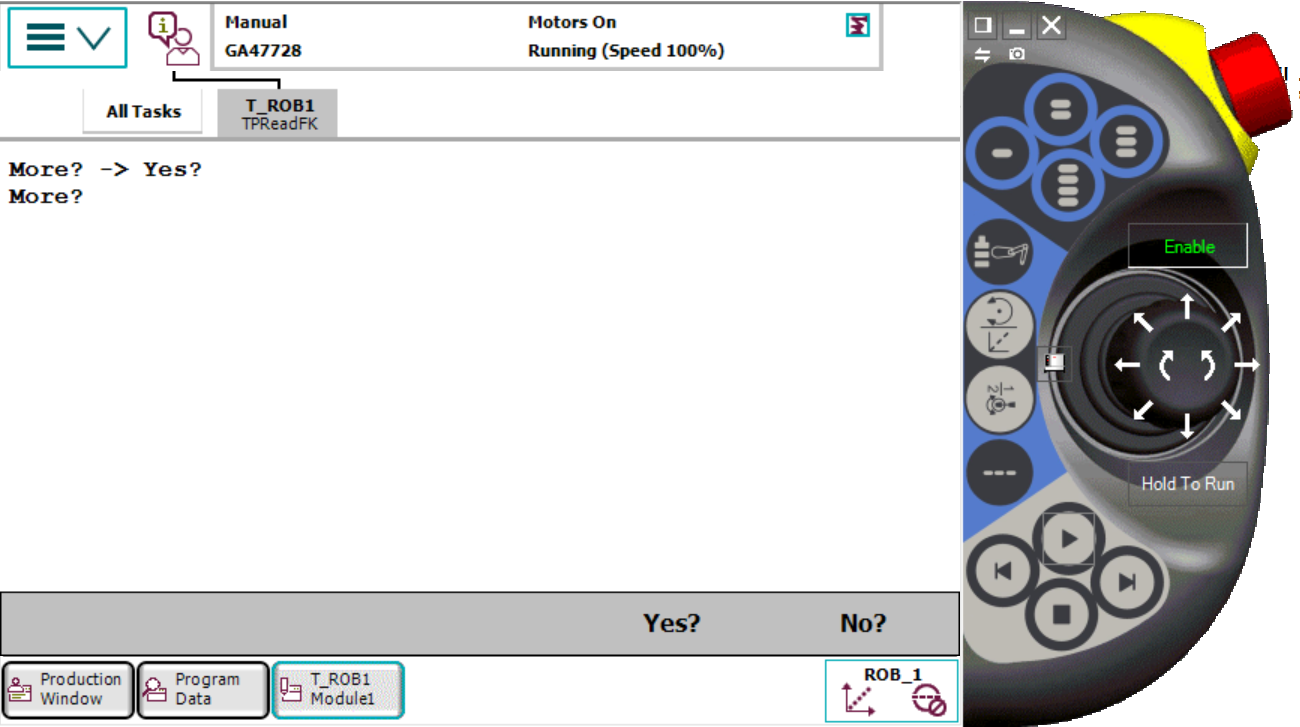
\includegraphics[width=1\textwidth]{i04861x37}

Beskrivelse av TPReadNum: TPReadNum (FlexPendant Read Numerical) blir
brukt til å lese ett nummer fra flexpendanten.

\begin{lstlisting}[basicstyle={\sffamily}]
TPReadNum reg1, "How many units should be produced?";
\end{lstlisting}

Teksten \textquotedblleft How many units should be produced?\textquotedblright{}
vil bli skrevet på flexpendant skjermen. Programmet vil ikke fortsette
før det har blitt lagt inn ett tall på det numeriske tastaturet. Tallet
vil bli lagret i Reg1.
\end{enumerate}

\textbf{Arbeidsoppdrag 4 - Programmering II}

\textbf{Stabling av klosser.}
\begin{enumerate}
\item Definer verktøy og workobjecter. 
\item Lag rutiner for Init, Åpne- og Lukkegriper, Hent- og Leverpuck. 
\item Lag Meny rutine til å velge fra hvilken stabel en skal hente. 
\item Bruk navn på Robtarget f.eks pHentHvitKloss. 
\item En skal hente fra 2 posisjoner og stable i høyden (1 stabel). 
\item Bruk TPReadNum til å bestemme antall klosser levert i høyden.
\end{enumerate}

\textbf{Offs}

Offs is used to add an offset in the object coordinate system to a
robot position.

Example 1:

\begin{lstlisting}[basicstyle={\sffamily}]
MoveL Offs(p2, 0, 0, 10), v1000, z50, tool1;
\end{lstlisting}

The robot is moved to a point 10 mm from the position p2 (in the z-direction).

Example 2

\begin{lstlisting}[basicstyle={\sffamily}]
p1 := Offs (p1, 5, 10, 15);
\end{lstlisting}

The robot position p1 is displaced 5 mm in the x-direction, 10 mm
in the y-direction and 15 mm in the z-direction.
\begin{enumerate}
\item Lever klosser i 4 stabler ved å bruke Offset i X og Y (et lag om gangen). 
\item Endre henteposisjonene fra 1 i høyden til å plukke fra stabel, hentehøyden
bestemmes ved å taste inn antall i meny rutinen. 
\item Lag operatørkommunikasjon som fortell at det er tomt for klosser i
hentepos og fullt i leveringsposisjoner.
\end{enumerate}
\newpage{}














\underbar{file i04861}
\vfil \eject
%(END_QUESTION)





%(BEGIN_ANSWER)


%(END_ANSWER)





%(BEGIN_NOTES)


%INDEX% Arbeisdoppdrag, Robot, Nivå 1, Stasjonr6, Jobbing og TCP

\textbf{Arbeidsoppdrag - Jogging og TCP}
%(END_NOTES)


